\runningheader{Oppgave g)}{}{Side \thepage\ av \numpages}



% ********************************************************
% oppgave g) 
% ********************************************************  
\item
  I denne oppgaven skal du implementere følgende 3 signal ved bruk av  
  en {\sf  Ramp}-blokk og to {\sf  Sine Wave}-blokker.
  \begin{align}
    v_{1}(t) & = 3.2\sin(1.2t)+2 \\
    v_{2}(t) & =
 \begin{cases}%
  1 &\text{for } 0\leq t<15~ \text{sekund}\\
   1+0.3{\cdot}(t-15)   & \text{for } t \geq 15 ~ \text{sekund} 
 \end{cases}\\
    v_{3}(t) & = 1.7\cos(0.7t)+3
  \end{align}
 Legg merke til at $v_{3}$ er et cosinus-signal. 
  Lag deretter et signal $u(t)$ som baserer seg på de 3 signalene på
  følgende måte. 
  \begin{equation}
    \label{eq:208a}
    u(t) = \frac{v_{1}(t)}{v_{2}(t){\cdot}v_{3}(t)} 
  \end{equation}
  Bruk kun én {\sf  Produkt}-blokk til å lage $u(t)$. Send alle 4
  signalene til et scope.
    {\color{red}La simuleringstiden fortsatt være 25 sekund.  }

      {\bf Gjør følgende oppgaver / svar på følgende spørsmål:    }
  \begin{enumerate}[label=g\arabic*)]
\item Bygg modellen og ta med skjermdump av den i innleveringen din.
  \item 
    Simuler modellen og ta med simuleringsresulatet
    i innleveringen din. Vis at du får en figur lik denne.

  \begin{figure}[H]
    \centering
    \hspace*{0mm}\scalebox{0.6}{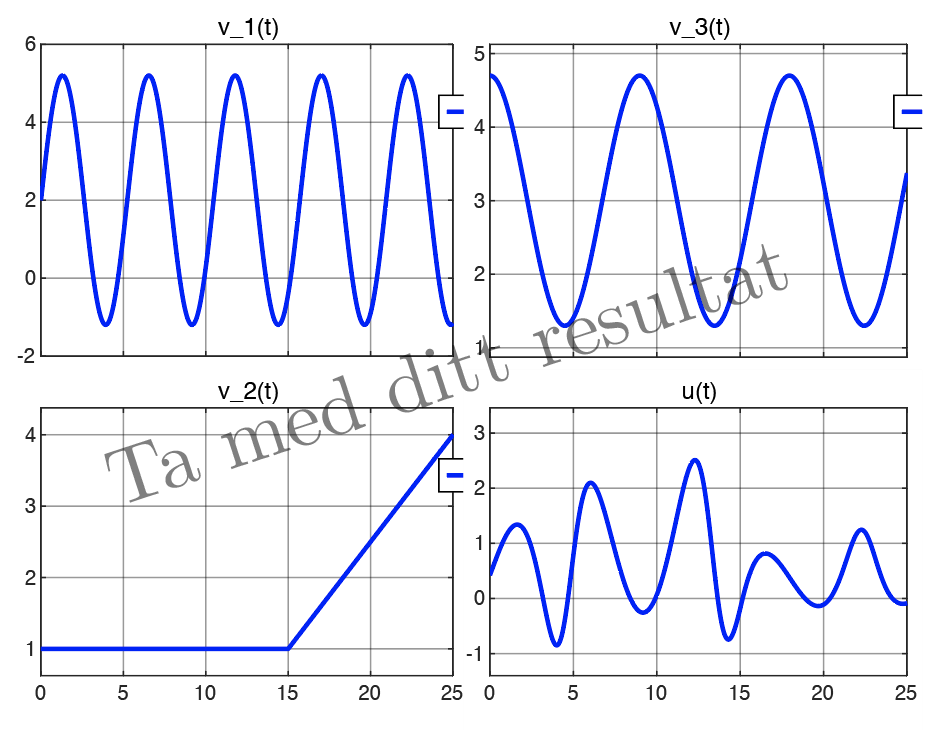
\includegraphics{fig_2g.png}}
    \caption{Simuleringsresultatet}
  \end{figure}

\item Velg et vilkårlig tidspunkt etter $t{=}15$ sekund og les av en verdi
fra $u(t)$. Sett inn samme 
tidspunkt i ligning~\eqref{eq:208a} innsatt $v_{1}(t)$, $v_{2}(t)$ og
$v_{3}(t)$,
og vis at resultatet stemmer med simuleringen. 

    \end{enumerate}
